Here are my plots of how well my implementation of the k-NN algorithm scores on the validation\footnote{I have chosen the validation set by randomly sampling 20 percent of the training set.} and test set for different K's. I have calculated the score as the fraction of correctly classified digits out of the total number of digits in the validation/test set. I know that the assignment text asked for the error, but I find this score measure more meaningful and therefore I have used that instead, since it does not make any difference for which K's are chosen: If the error is defined by just counting the number of misclassified points, then a K obtains a maximal score, if and only if it obtains a minimal error.

If the maximum score of all K's on the validation/test set is obtained by more than one K, then my implementation of the algorithm choses the median of these K's as the optimal K. This chosen optimal K is marked be the vertical, dotted lines.

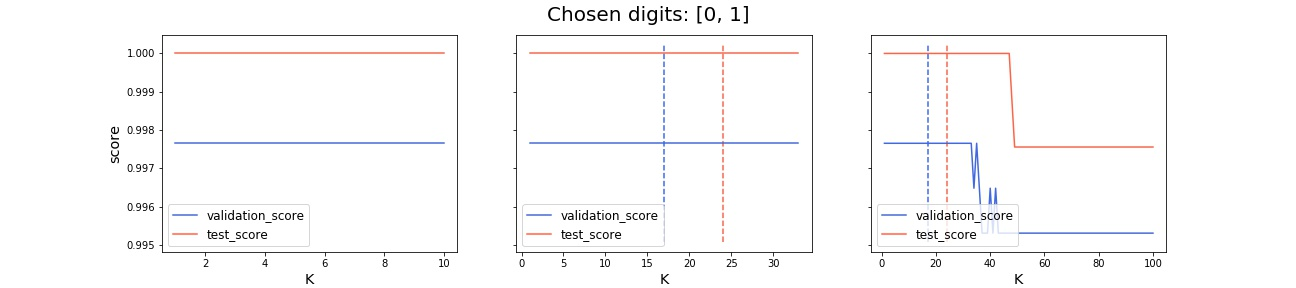
\includegraphics[scale = 0.3]{nearest_neighbour/digits_0_1.jpg}

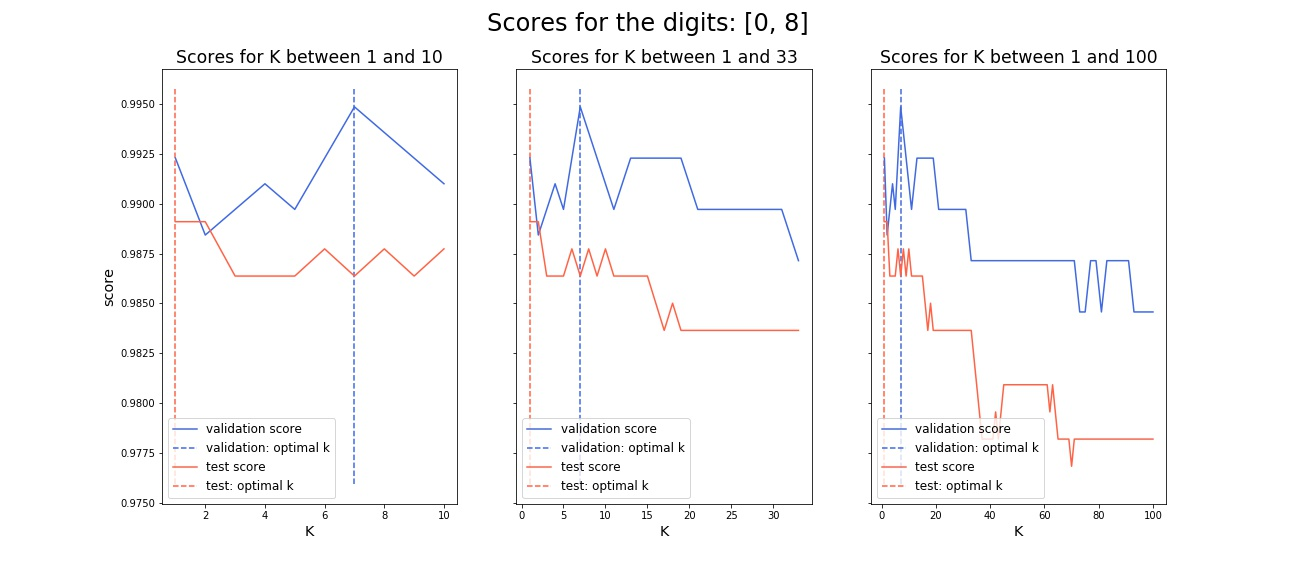
\includegraphics[scale = 0.3]{nearest_neighbour/digits_0_8.jpg}

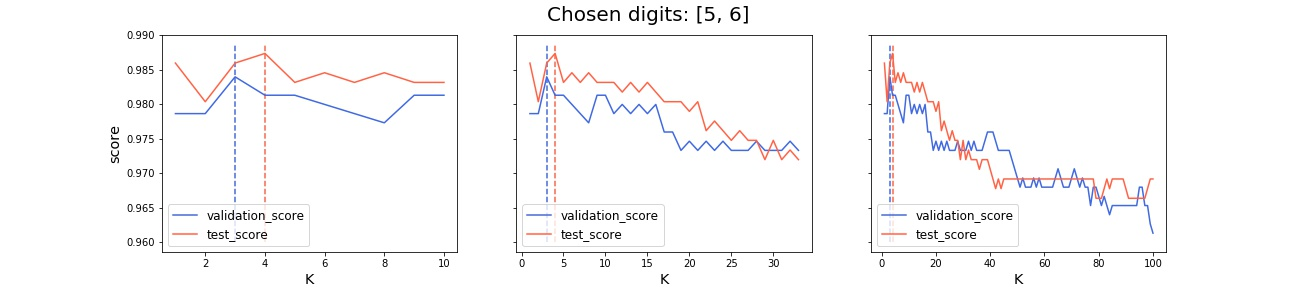
\includegraphics[scale = 0.3]{nearest_neighbour/digits_5_6.jpg}

Here is a table of the maximum scores and correspondingly chosen K for each of the digit pairs:

\begin{tabular}{lllll}
Digit pair & Val. max. score & Val. chosen K & Test max. score & Test chosen K \\
{[}0,1{]}  & 0.998                 & 17                  & 1.000           & 24            \\
{[}0,8{]}  & 0.995                 & 7                   & 0.989           & 1             \\
{[}5,6{]}  & 0.984                 & 3                   & 0.987           & 4            
\end{tabular}


First of all, if we look at the plots for the digit pair [0,1], then we see that we have many K's obtaining the maximum score, and therefore different strategies for choosing between tying K's would produce different choices of K. In my implementation, I choose the median of all optimal K's. 

Secondly, we see that for all the digits pair, the validation score approximates the test score quite well, but still the validation score do not point to exactly the same K as optimal as the test score for any of the digits pair. 

As a more general comment, we can note that that in this setup, where we are looking at the errors over all possible K's for both the validation and the test set, we are in fact using the validation and test set completely symmetricly, and none of them should be really be called a validation or test set. If we are not using the scores on any of the sets to choose a K for the future use of the algorithm, then the score for any given K on both sets is an unbiased estimate of how well the algorithm will perform, if choose this K for the future use of the algorithm. If we, however, use the validation set as an actual validation set to choose a K that obtains the maximum validation score over all the K's, then the validation score for this K is no longer an unbiased estimate of the future performance of the model, but an overestimate. This is because we are choosing not a random K, but exactly a K that performs optimally on the validation set, but a part of this optimal performance is just noise (it would disappear if we averaged over enough validation sets), and therefore we end up with an overestimate. However, we can now use the score for this K on the test set (the intersection of the dotted blue line and the orange curve) as an unbiased estimate of the future performance of the algorithm. If we do that, we get the following chosen K's and unbiased performance estimates:

\begin{tabular}{lll}
Digit pair & Val. chosen K & Test score for this K \\
{[}0,1{]}  & 17                  & 1.000                 \\
{[}0,8{]}  & 7                   & 0.986                 \\
{[}5,6{]}  & 3                   & 0.986                
\end{tabular}